\documentclass[aspectratio=169]{beamer}

% beamer config
\usetheme{Berkeley}
% \AtBeginSection{\frame{\sectionpage}}

% package imports
\usepackage{graphicx}
\graphicspath{{./figs/}}

% Macros
\newcommand{\todo}[1]{\textcolor{red}{\textbf{[#1]}}}

\title[PhotoHunter]{PhotoHunter: A Citizen-Scientist Game with User-in-the-loop
  Data Confirmation for Collecting Computer Vision Datasets of
  Geo-tagged Imagery through Crowd-Sourcing Data Collection;
  Abstracting Research using an Interactive, Game-based Mobile
  Application for Large Dataset Creation}

\author[]{Connor Greenwell \and Ryan Baltenberger
  \and J.\ David Smith \and Aaron Bradshaw}

\institute{QuesoTech.com}

\begin{document}

\maketitle

\section{Overview}

\begin{frame}{System Overview}
  \centering
  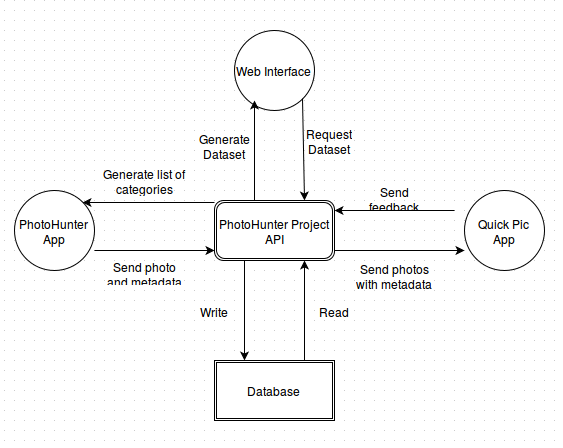
\includegraphics[width=\textwidth,height=\textheight,keepaspectratio]{ss_flowchart}
\end{frame}

\subsection{Researchers Interface}

\begin{frame}{Researchers Interface}
  \centering
	\todo{update this picture}
  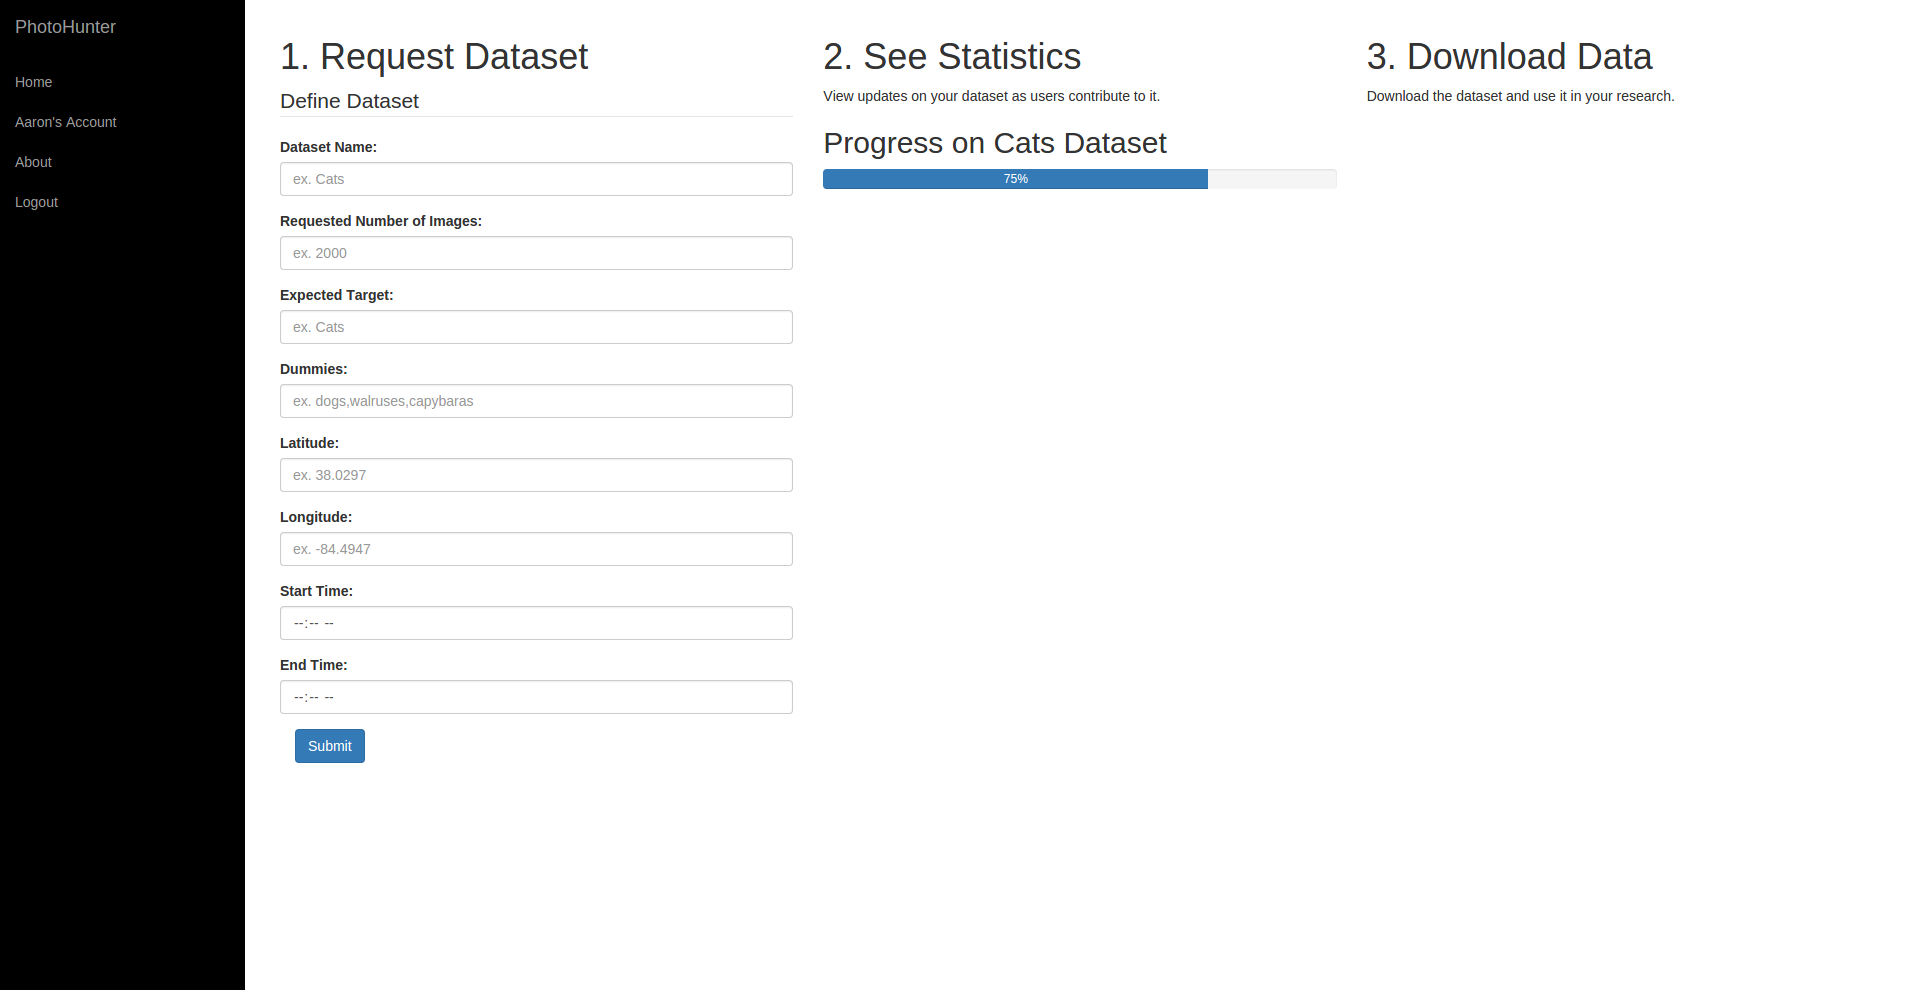
\includegraphics[width=\textwidth,height=\textheight,keepaspectratio]{researchers}
\end{frame}

\subsection{PhotoHunter}

\begin{frame}{PhotoHunter}
  \begin{columns}[c]
    \begin{column}{0.5\columnwidth}
      \centering
      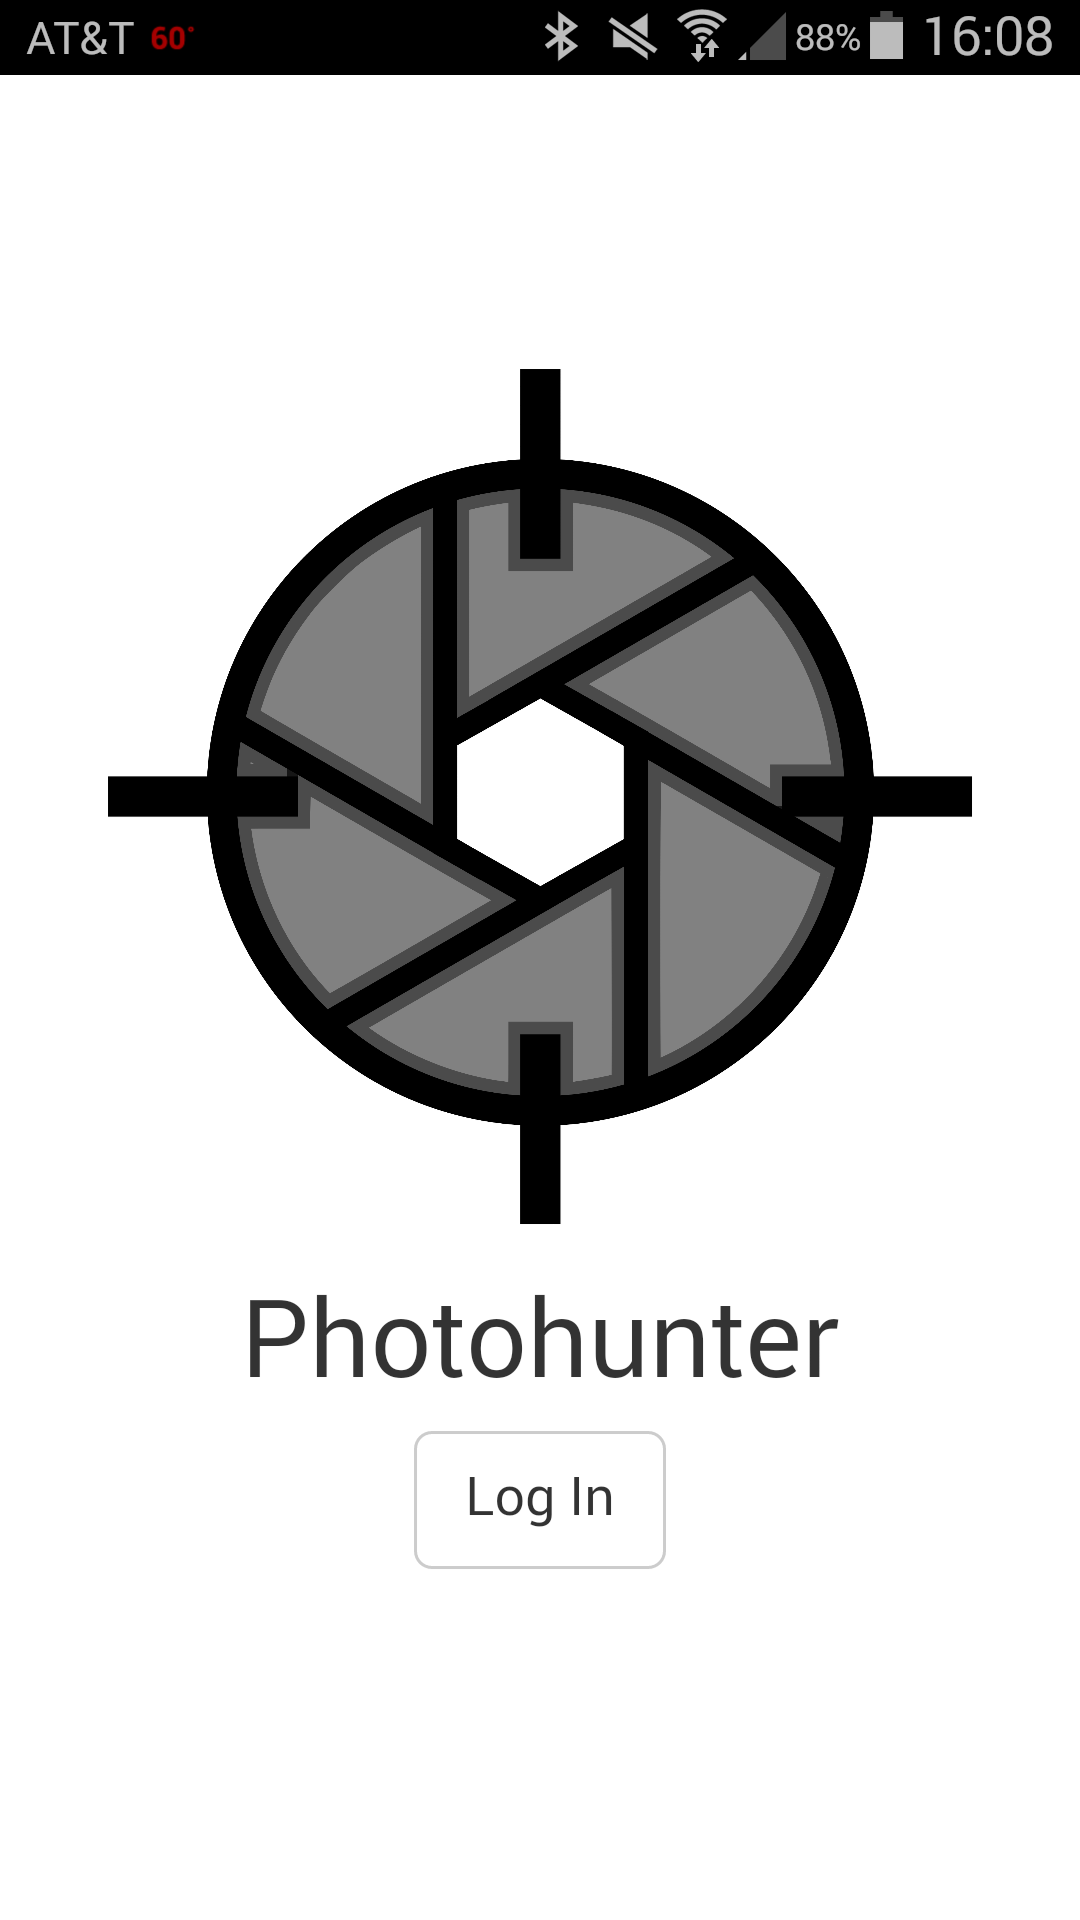
\includegraphics[width=\textwidth,height=\textheight,keepaspectratio]{photohunter/login}
    \end{column}
    \begin{column}{0.5\columnwidth}
      \centering
      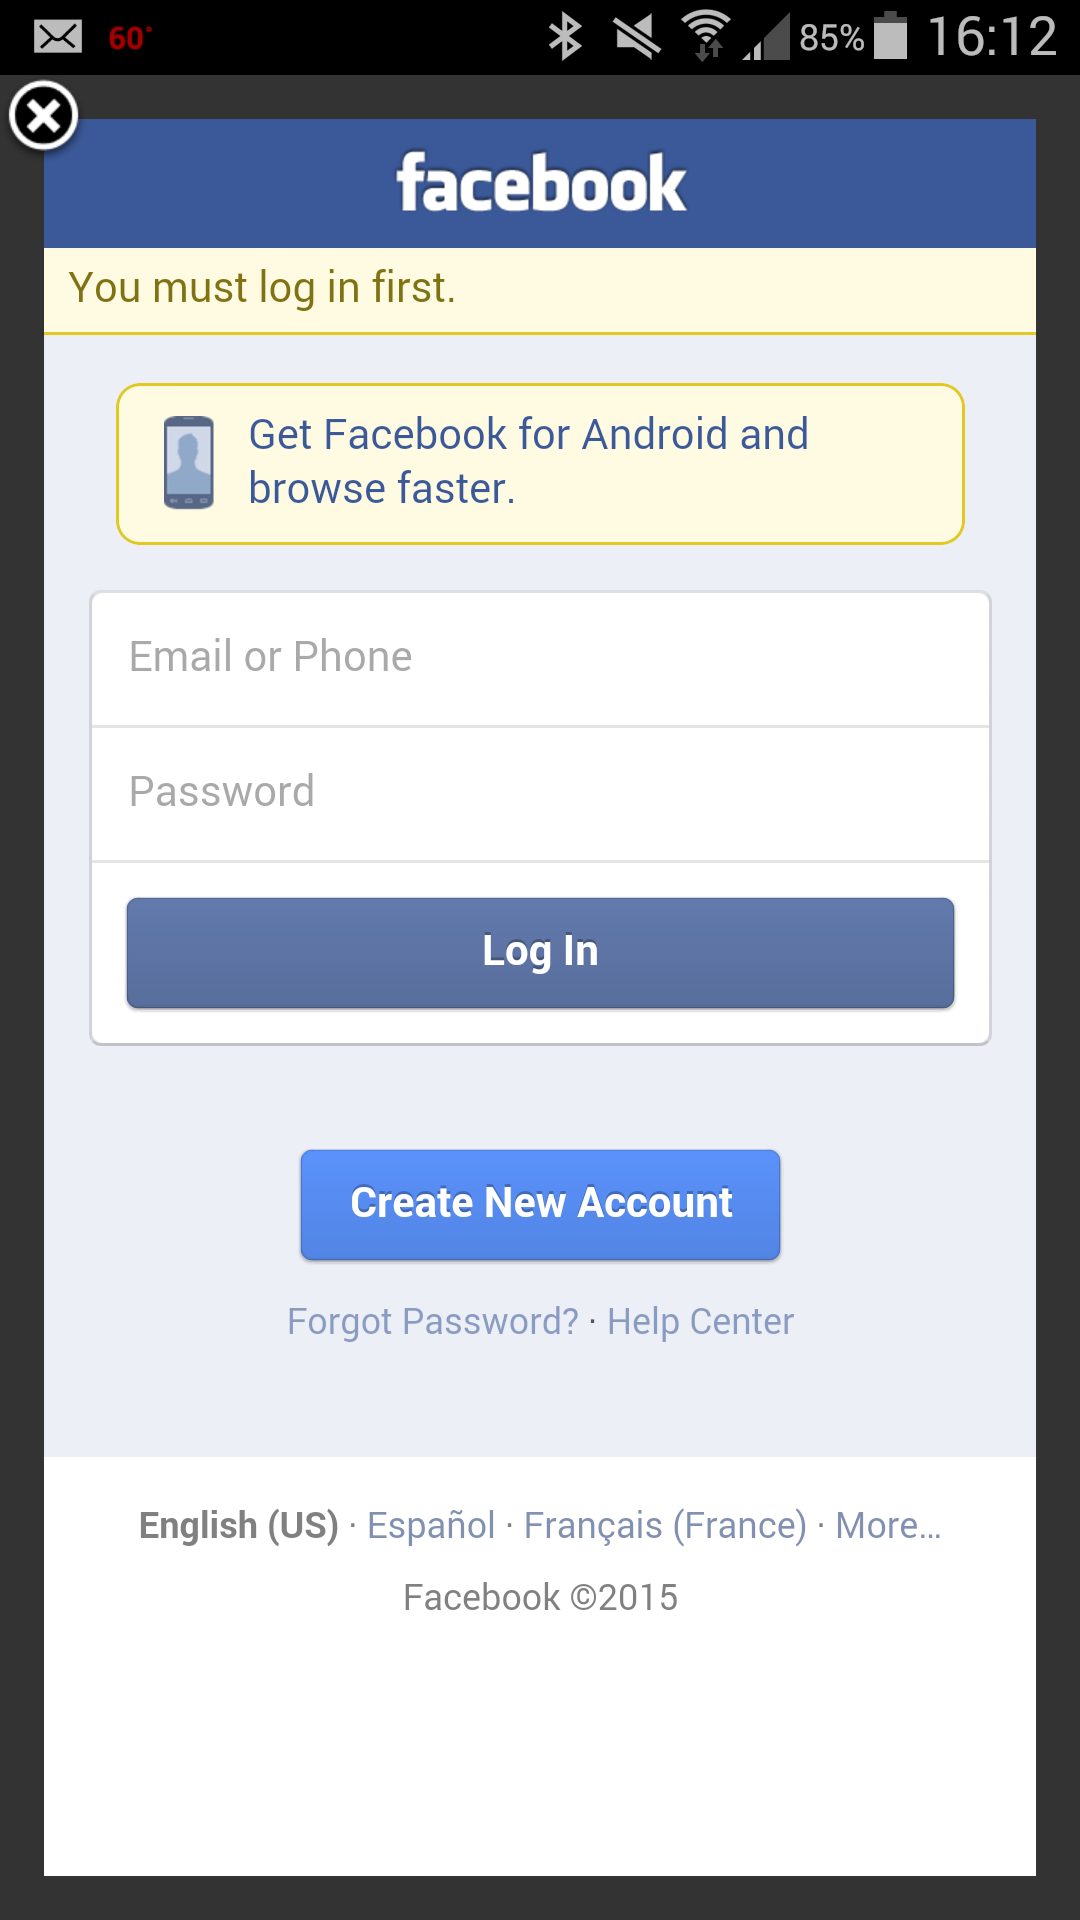
\includegraphics[width=\textwidth,height=\textheight,keepaspectratio]{photohunter/fb}
    \end{column}
  \end{columns}
\end{frame}

\begin{frame}{PhotoHunter}
  \begin{columns}[c]
    \begin{column}{0.3\columnwidth}
      \centering
      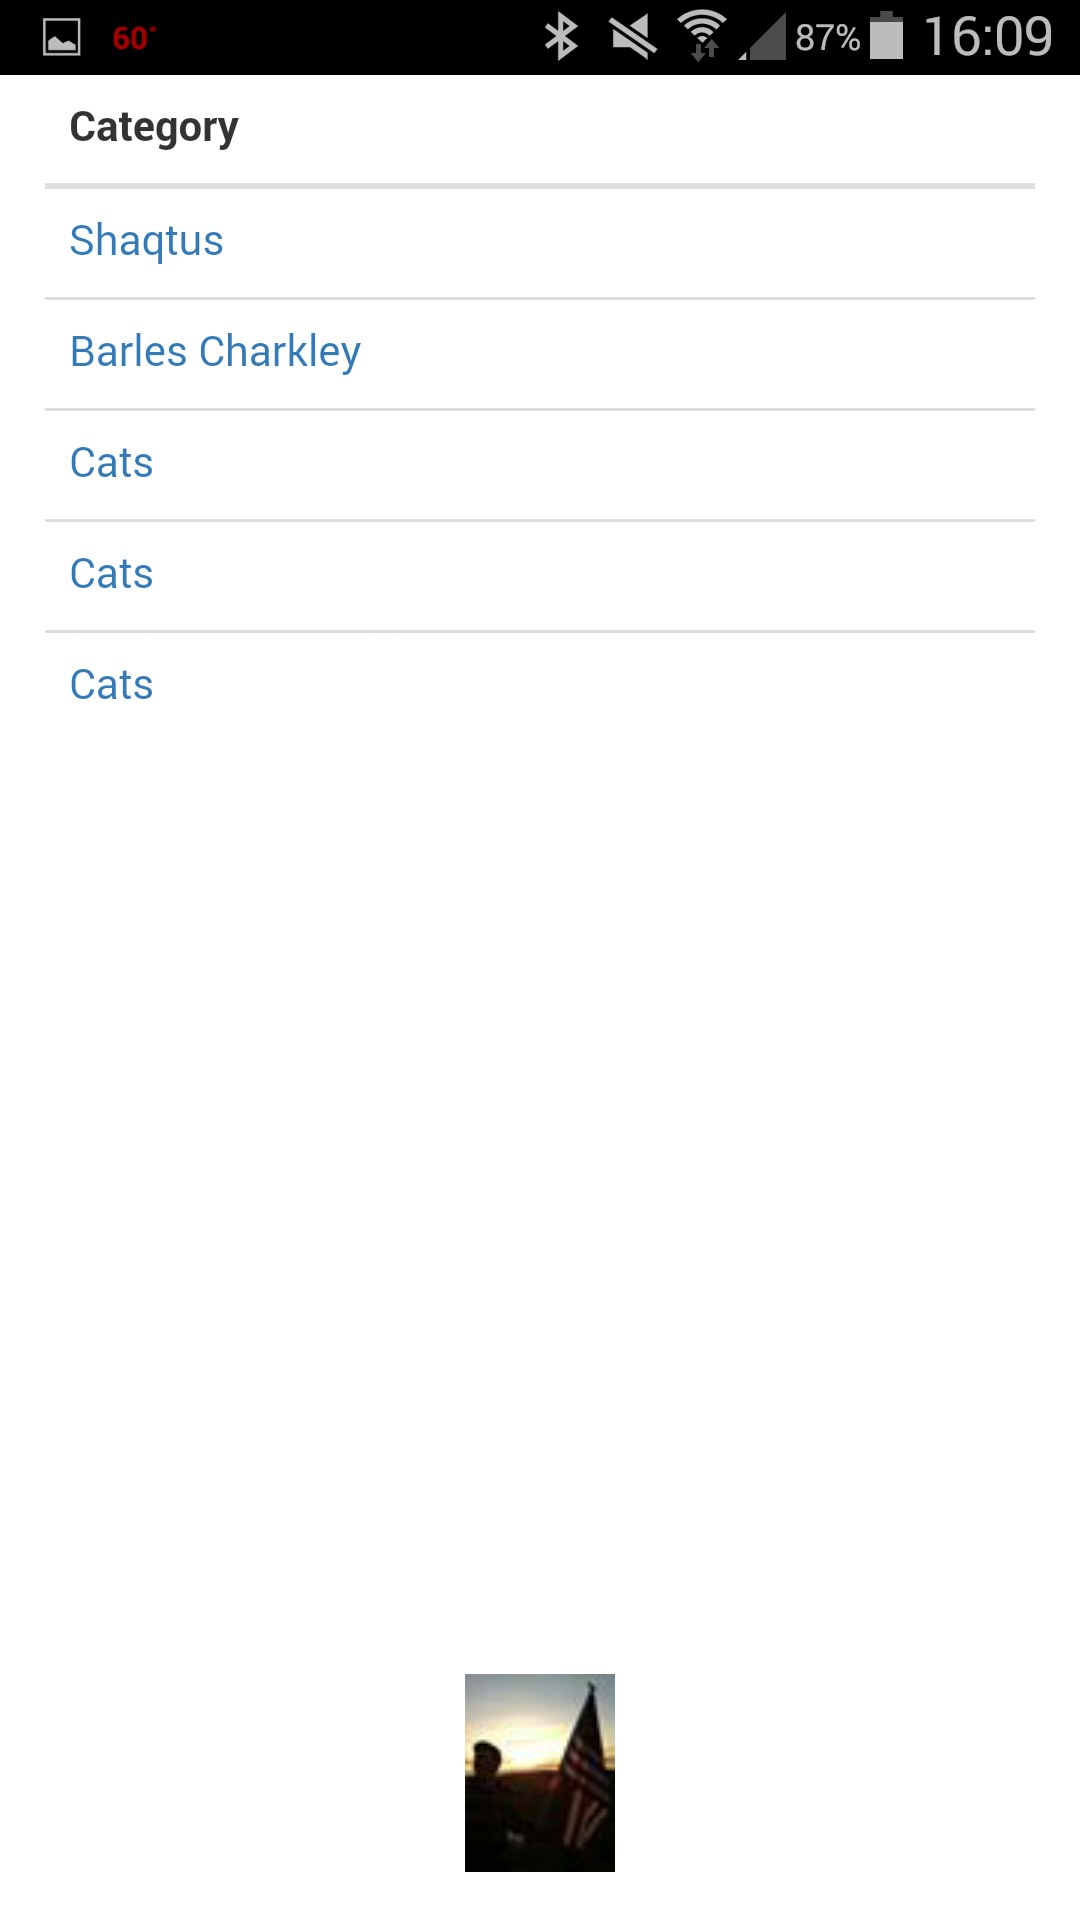
\includegraphics[width=\textwidth,height=\textheight,keepaspectratio]{photohunter/list}
    \end{column}
    \begin{column}{0.3\columnwidth}
      \centering
      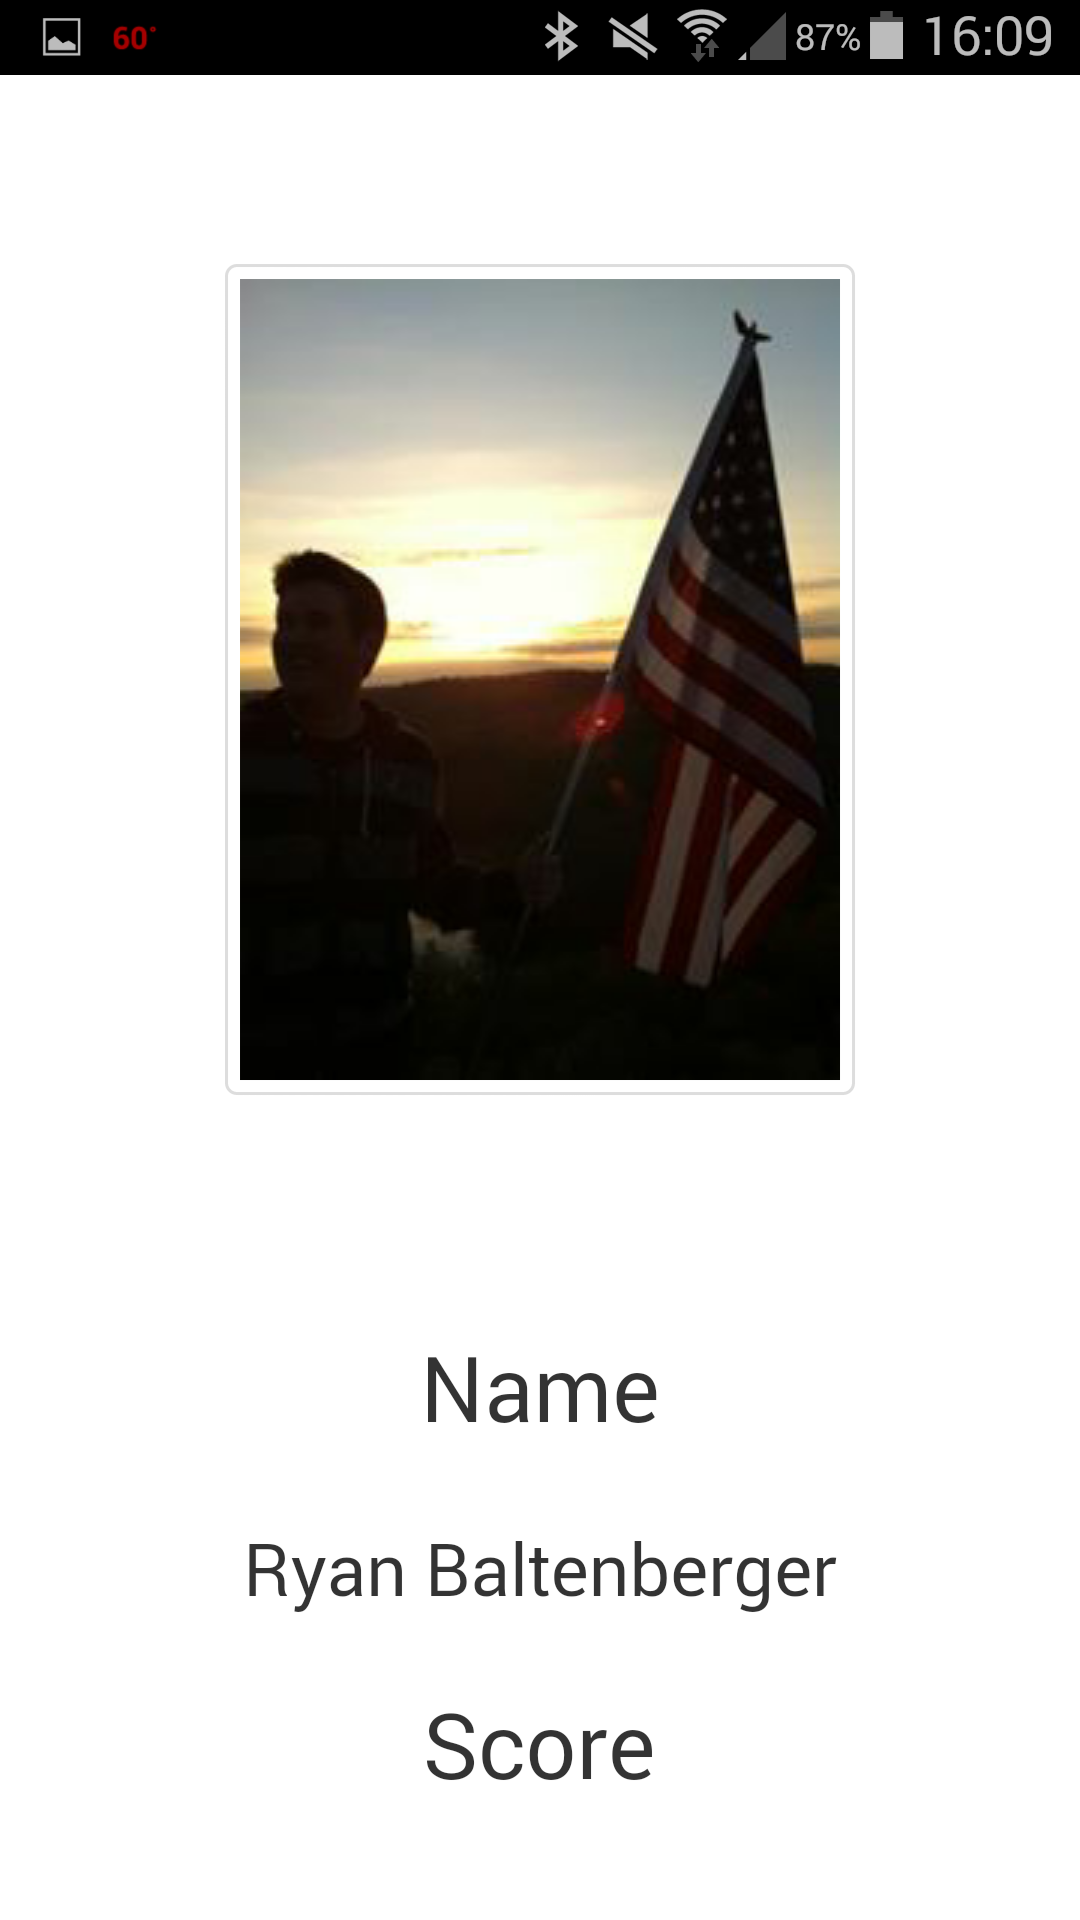
\includegraphics[width=\textwidth,height=\textheight,keepaspectratio]{photohunter/user}
    \end{column}
    \begin{column}{0.3\columnwidth}
      \centering
      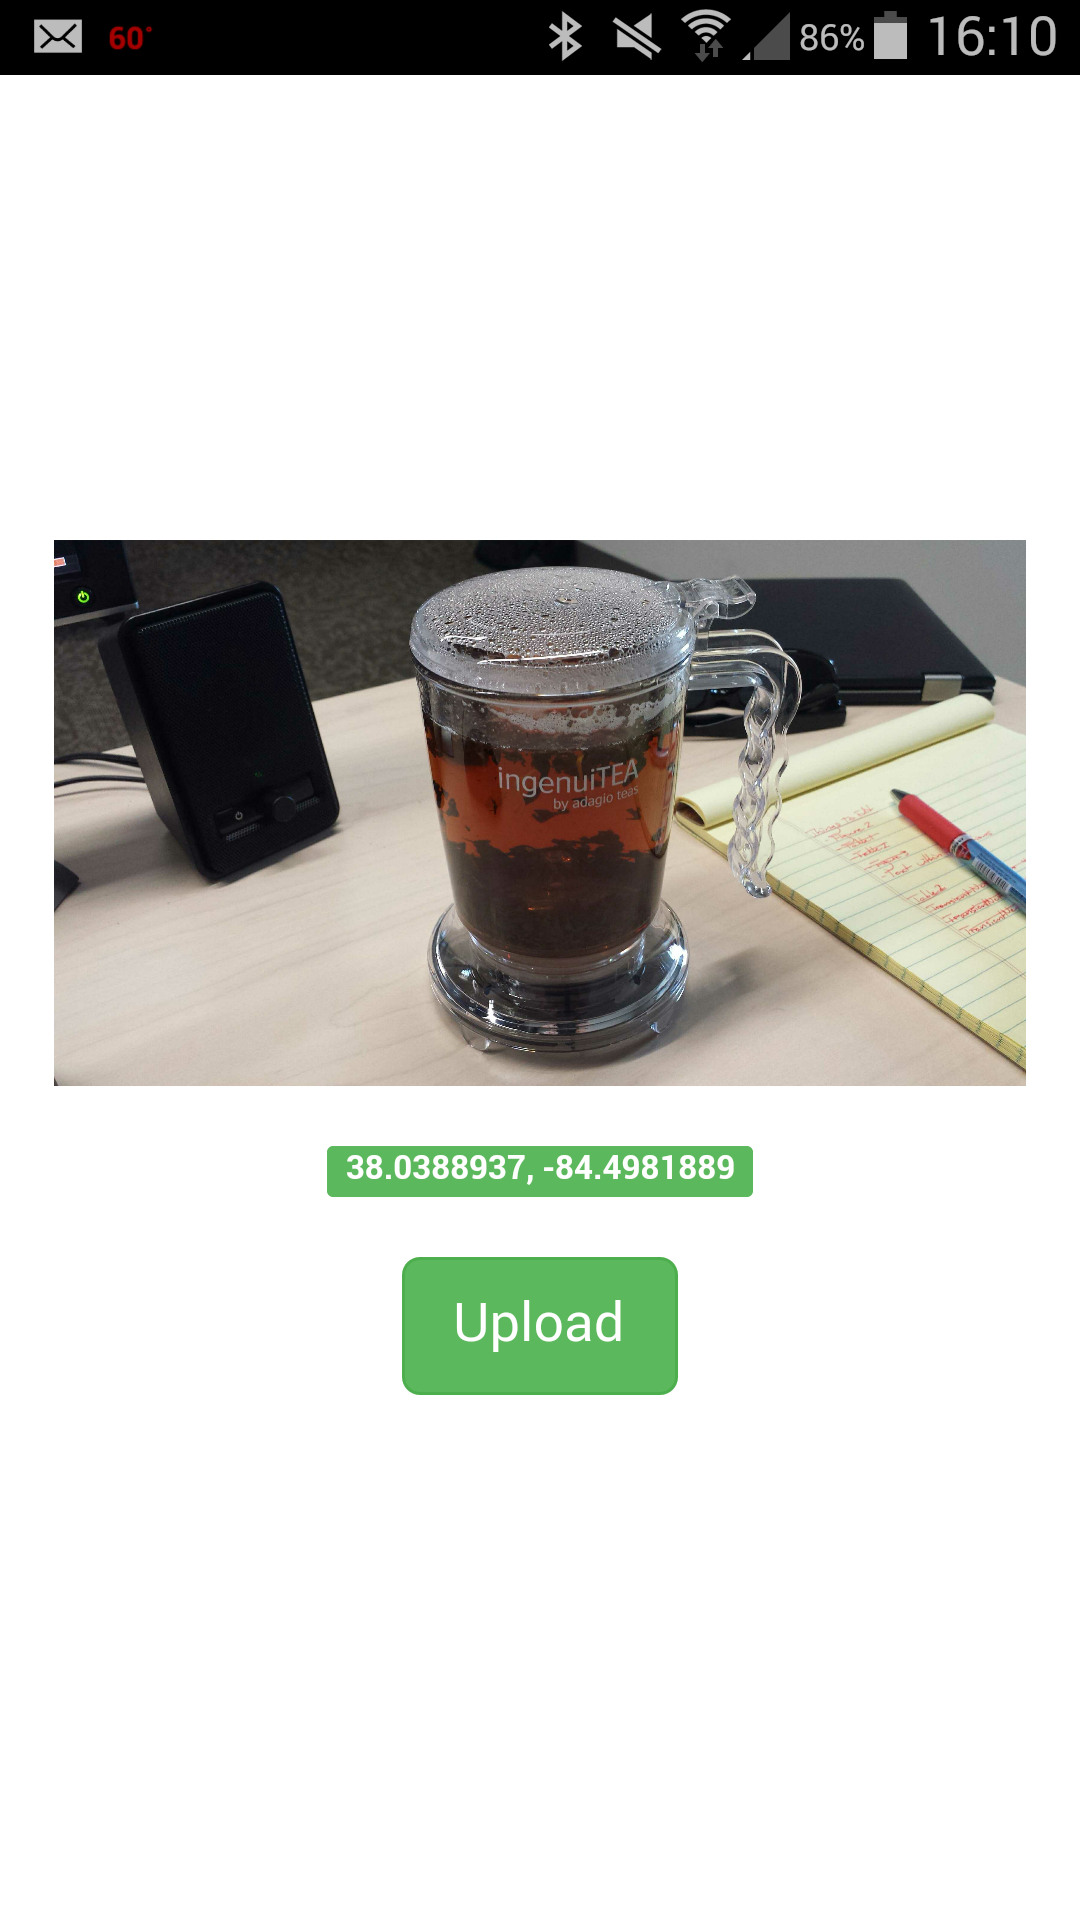
\includegraphics[width=\textwidth,height=\textheight,keepaspectratio]{photohunter/submit}
    \end{column}
  \end{columns}
\end{frame}

\subsection{QuickPic}

\begin{frame}{QuickPic}
  \begin{columns}[c]
    \begin{column}{0.5\columnwidth}
      \centering
			\todo{add in updated screenshots}
      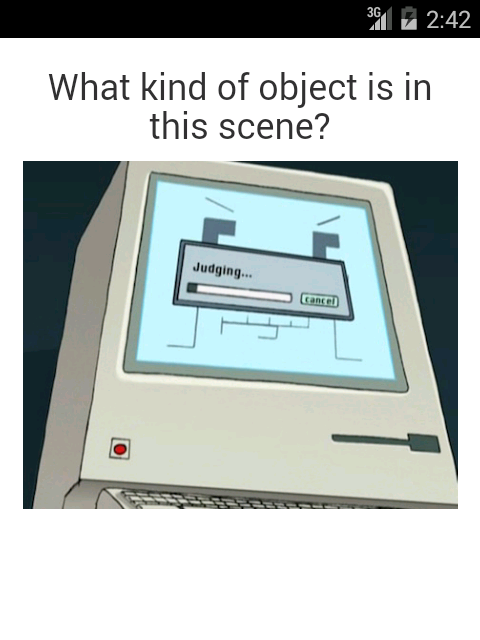
\includegraphics[width=\textwidth,height=\textheight,keepaspectratio]{ss_quickpic_image}
    \end{column}
    \begin{column}{0.5\columnwidth}
      \centering
			\todo{add in updated screenshots}
      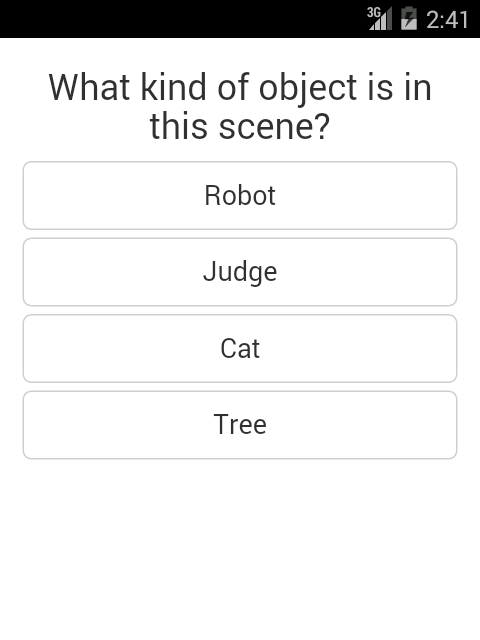
\includegraphics[width=\textwidth,height=\textheight,keepaspectratio]{ss_quickpic_options}
    \end{column}
  \end{columns}
\end{frame}

\subsection{Backend}

\begin{frame}{ER Diagram}
  \centering
  \includegraphics[width=\textwidth,height=\textheight,keepaspectratio]{er}
\end{frame}

% Discuss problems, and your solutions
\section{Problems}

% Discuss lessons learned while doing the project
\section{Lessons Learned}

% Discuss your initial assumptions about the project compared to what you know now
\section{Assumptions}

% Does the project match what the customer initially wanted, how did it evolve
\section{Evolution}

% Changes requested by the customer, or changes to specifications due to implementation
\section{Changes}

% Discuss future enhancements, usage
\section{The Future!}

\frame{\centering Thanks!}

\end{document}
